\documentclass{article}
\usepackage[hyphens]{url}
\usepackage{mathtools}
\usepackage{amsmath}
\usepackage{listings}
\usepackage{graphicx}
\usepackage[margin=1in]{geometry}
\usepackage{float}
\floatstyle{boxed}
\restylefloat{figure}
\lstset{basicstyle=\footnotesize, breaklines=true}
\begin{document}


\title{CS595 Intro to Web Science, Assignment \#10}
\author{Valentina Neblitt-Jones}
\date{December 12, 2013}
\maketitle

\newpage
\listoftables
\lstlistoflistings
\listoffigures

\newpage
\section*{Question 1}

Choose a blog or newsfeed (or something with an Atom or RSS feed). It should be on a topic or topics or which you are qualified to provide classification training data. Find something with at least 100 entries. \\

Create between four and eight different categories for the entries in the feed: \\

examples: \\

work, class, family, news, deals \\

liberal, conservative, moderate, libertarian \\

sports, local, financial, national, international, entertainment \\

metal, electronic, ambient, folk, hip-hop, pop \\

Download and process the pages of the feed as per the week 12 class slides.

\subsection*{Answer to Question 1}

%\begin{figure}[H]
%\centering
%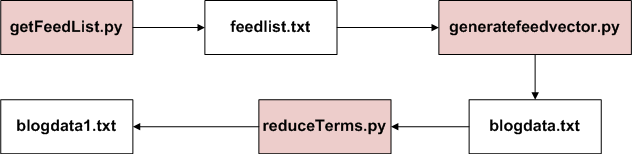
\includegraphics[scale=0.50]{q01/FlowForQ1}
%\caption{Creation of the Blog-Term Matrix}
%\label{FlowForQ1}
%\end{figure}

\newpage
\section*{Question 2}
Manually classify the first 50 entries, and then classify (using the fisher classifier) the remaining 50 entries. Report the cprob() values for the 50 titles as well. From the title or entry itself, specify the 1-, 2-, or 3-gram that you used for the string to classify. Do not repeat strings; you will have 50 unique strings. For example, in these titles the string used is marked with *s: \\

\begin{itemize}
\item *Rachel Goswell* - ``Waves are Universal'' (LP Review)
\item The *Naked and Famous* - ``Passive Me, Aggressive You'' (LP Review)
\item *Negativland* - ``Live at Lewis's, Norfolk VA, November 21, 1992'' (concert)
\item Negativland - ``*U2*'' (LP Review)
\end{itemize}

Note how 	``Negativland'' is not repeated as a classification string. \\

Create a table with the title, the string used for classification, cprob(), predicted category, and actual category.

\subsection*{Answer to Question 2}

%\begin{lstlisting}[frame=single, caption=generateImages.py, label=generateImages]
%\end{lstlisting}

%\begin{table}[!h]
%\centering
%\begin{tabular}{c c}
%Value of k & No. of Iterations \\
%\hline
%5 & 6  \\
%10 & 7  \\
%20 & 100  \\
%\hline
%\end{tabular}
%\caption{K-Means Iterations}
%\end{table}

\newpage
\section*{Question 3}

\subsection*{Answer to Question 3}

Assess the performance of your classifier in each of your categories by computing precision and recall. Note that the definitions are slightly different in the context of classification; see: \url{http://en.wikipedia.org/wiki/Precision_and_recall#Definition_.28classification_context.29}

%\begin{lstlisting}[frame=single, caption=getKMeans.py, label=getKMeans]
%\end{lstlisting}

%\begin{itemize}
%\item Blonde Ambition
%\item ups
%\item Alcorn Studios
%\item All Scattered
%\end{itemize}

\newpage

\section*{Question 4 - Extra Credit (5 points)}

Redo the questions above, but with the extensions on slide 26 and pp. 136-138.

\subsection*{Answer to Question 4}

Not attempted.

%\renewcommand\thesubsection{\arabic{subsection}}
%\subsection{What 5 movies have the highest average ratings? Show the movies and their ratings sorted by their average ratings.}

%\begin{lstlisting}[frame=single, caption=highestavgrating.py, label=highaverage]
%\end{lstlisting}

%\newpage
%\subsection{What 5 movies have received the most ratings? Show the movies and the number of ratings sorted by number of ratings.}

%\begin{table}[!h]
%\centering
%\begin{tabular}{l c}
%Movie Title & No. of Ratings \\
%\hline
%Star Wars (1977) & 583  \\
%Contact (1997) & 509  \\
%Fargo (1996) & 508  \\
%Return of the Jedi (1983) & 507  \\
%Marlene Dietrich: Shadow and Light (1997) & 485  \\
%\hline
%\end{tabular}
%\caption{Movies with the Most Ratings}
%\end{table}

%\begin{figure}[H]
%\centering
%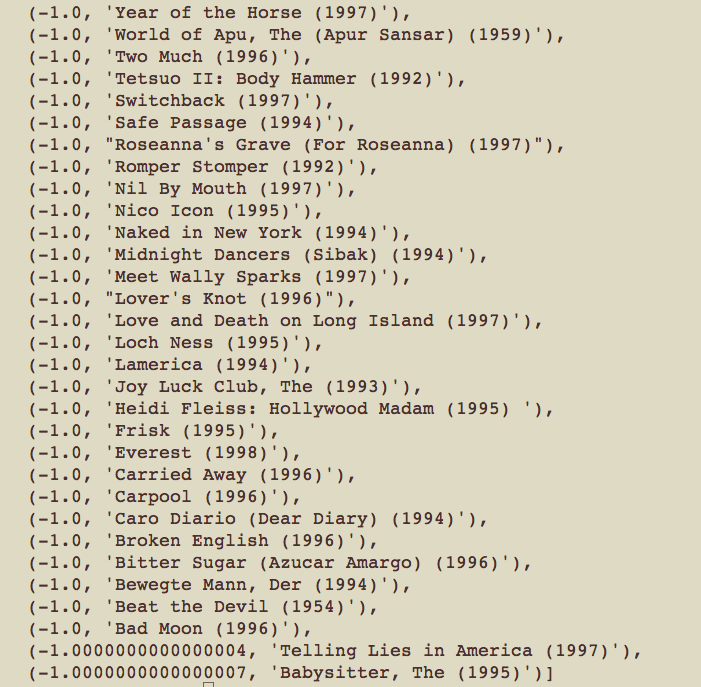
\includegraphics[scale=0.50]{q05/leastliketopgun}
%\caption{Movies Least Like Top Gun}
%\label{leastliketopgun}
%\end{figure}

\newpage
\appendix

\section{getFeedList.py}

%\begin{lstlisting}[frame=single, caption=getFeedList.py, label=getFeedList]
%\end{lstlisting}

\section{generatefeedvector.py}

%\begin{lstlisting}[frame=single, caption=generatefeedvector.py, label=generatefeedvector]
%\end{lstlisting}

\section{reduceTerms.py}

%\begin{lstlisting}[frame=single, caption=reduceTerms.py, label=reduceTerms]
%\end{lstlisting}

\section{clusters.py}

%\begin{lstlisting}[frame=single, caption=clusters.py, label=clusters]
%\end{lstlisting}

\section{Output from getKMeans.py}

%\begin{lstlisting}[frame=single, caption=kmeansoutput.txt, label=kmeansoutput]
%\end{lstlisting}

\section{Output from getMDS.py}

%\begin{lstlisting}[frame=single, caption=MDSoutput.txt, label=MDSoutput]
%\end{lstlisting}

\newpage

\bibliographystyle{acm}
\bibliography{references}

\end{document}